% arara: pdflatex
% arara: biber
% arara: pdflatex
% arara: pdflatex

\documentclass[8pt]{article}
\usepackage[affil-it]{authblk}

\renewcommand{\thefigure}{S\arabic{figure}}

\usepackage{mathrsfs}
\usepackage{fullpage}
\usepackage{amssymb}
\usepackage{graphicx}
\usepackage{amsmath}
\usepackage[usenames,dvipsnames]{xcolor}
\usepackage[strict]{changepage}
\usepackage{framed}
\usepackage{amsthm}
\usepackage{bbm}
\usepackage{colortbl}
\usepackage{epsfig}


\DeclareMathOperator{\diag}{diag}
\DeclareMathOperator{\Tr}{\mbox{Tr}}
\DeclareMathOperator{\tr}{\mbox{tr}}
\DeclareMathOperator{\re}{\mbox{Re}}
\DeclareMathOperator{\im}{\mbox{Im}}
\DeclareMathOperator{\erfc}{{erfc}}
\DeclareMathOperator{\sign}{{sign}}

\newcommand{\mkch}[1]{{\color{RoyalBlue} MK: #1}}
\newcommand{\bcch}[1]{{\color{BrickRed} BC: #1}}

\newcommand{\ch}{Ch.\@\xspace}
\newcommand{\se}{Sec.\@\xspace}
\newcommand{\Se}{Sec.\@\xspace}
\newcommand{\app}{App.\@\xspace}
\newcommand{\ie}{i.e.\@\xspace}
\newcommand{\eg}{e.g.\@\xspace}

\newcommand{\mean}[1]{\langle #1 \rangle_m}
\newcommand{\ptl}{\partial}
\newcommand{\DF}[2]{\frac{d\, #1}{d\, #2}}
\newcommand{\PDF}[2]{\frac{\ptl\, #1}{\ptl\, #2}}
\newcommand{\PDFS}[2]{\frac{\ptl^2}{\ptl\, #1 \ptl\, #2}}
\newcommand{\DELF}[2]{\frac{\delta\,#1}{\delta\,#2}}
\newcommand{\ve}[1]{{\bf #1}}
\newcommand{\mat}[1]{\mathsf{#1}}
\newcommand{\nag}{{\phantom{\dagger}}}
\newcommand{\dimmu}{t^{1/2}\delta^{3/2}}
\newcommand{\den}{\rho}

\newcommand{\eqw}[1]{(\ref{#1})}
\newcommand{\eq}[1]{Eq.\thinspace{}(\ref{#1})}
\newcommand{\eqq}[2]{Eqs.\thinspace{}(\ref{#1}) and (\ref{#2})}
\newcommand{\eqqs}[2]{Eqs.\thinspace{}(\ref{#1}) and (\ref{#2})}
\newcommand{\eqqqs}[3]{Eqs.\thinspace{}(\ref{#1}), (\ref{#2}) and (\ref{#3})}
\newcommand{\eqqqqs}[4]{Eqs.\thinspace{}(\ref{#1}), (\ref{#2}), (\ref{#3}) and (\ref{#4})}
\newcommand{\Eq}[1]{Eq.\thinspace{}(\ref{#1})}

\newcommand{\tab}[1]{Tab.\thinspace{}\ref{#1}}

\newcommand{\alg}[1]{Alg.\thinspace{}\ref{#1}}
\newcommand{\algline}[1]{\ref{#1}:}

\newcommand{\fig}[1]{Fig.\thinspace{}\ref{#1}}
\newcommand{\figg}[2]{Fig.\thinspace{}\ref{#1} and \ref{#2}}
\newcommand{\fc}[1]{({#1})}
\newcommand{\figc}[2]{Fig.\thinspace{}\ref{#1}\thinspace{}\fc{#2}}
\newcommand{\figcc}[3]{Fig.\thinspace{}\ref{#1}\thinspace{}\fc{#2} and \fc{#3}}
\newcommand{\Fig}[1]{Figure \ref{#1}}
\newcommand{\Figg}[2]{Figures \ref{#1} and \ref{#2}}
\newcommand{\Figc}[2]{Figure \ref{#1}\thinspace{}\fc{#2}}
\newcommand{\Figcc}[3]{Figure \ref{#1}\thinspace{}\fc{#2} and \fc{#3}}

\renewcommand{\d}{\ket{\downarrow}}
\renewcommand{\u}{\ket{\uparrow}}
\newcommand{\g}{\ket{g}}
\newcommand{\psk}[1]{\ket{\psi(#1)}}
\newcommand{\phk}[1]{\ket{\phi(#1)}}
\newcommand{\psb}[1]{\bra{\psi(#1)}}
\newcommand{\phb}[1]{\bra{\phi(#1)}}
\newcommand{\mun}{\delta \mu_n^\text{ec}}
\newcommand{\mup}{\delta \mu_p^\text{ec}}
\newcommand{\RR}{\ve R}
\newcommand{\CC}{\mathcal{C}}
\newcommand{\dd}{\mathrm{d}}
\newcommand{\diff}{\mathop{}\!\mathrm{d}}
\newcommand{\Shat}{\hat{\mathbf{S}}}
\newcommand{\shat}{\hat{S}}
\renewcommand{\sp}{\ket{\text{sp}(\ve{Q})}}
\newcommand{\KC}{K${}_3$C${}_{60}$ }

\def\bra#1{\mathinner{\langle{#1}|}}
\def\ket#1{\mathinner{|{#1}\rangle}}
\def\braket#1{\mathinner{\langle{#1}\rangle}}
\def\Bra#1{\left<#1\right|}
\def\Ket#1{\left|#1\right>}


% fancy indented paragraphs
\definecolor{formalshade}{rgb}{0.95,0.95,1}

\newenvironment{formal}{%
\def\FrameCommand{%
\hspace{1pt}%
{\color{blue}\vrule width 2pt}%
{\color{formalshade}\vrule width 4pt}%
\colorbox{formalshade}%
}%
\MakeFramed{\advance\hsize-\width\FrameRestore}%
\noindent\hspace{-4.55pt}% disable indenting first paragraph
\begin{adjustwidth}{}{7pt}%
\vspace{2pt}\vspace{2pt}%
}
{%
\vspace{2pt}\end{adjustwidth}\endMakeFramed%
}

\newtheorem{defn}{Definition}
\newtheorem{corr}{Corrolary}
\newtheorem{lemma}{Lemma}
\newtheorem{thm}{Theorem}
\newtheorem{remark}{Remark}
\newtheorem{notation}{Notation}
\sloppy
% Ben
\usepackage[backend=biber,style=nature, autocite=superscript, natbib=true]{biblatex}
\addbibresource{../mbl_references_v6.bib}

\usepackage[margin=0.5in]{geometry}
\usepackage[T1]{fontenc}
\usepackage[utf8]{inputenc}
\usepackage{graphicx}
\usepackage{multirow, multicol}
\usepackage{amstext,amsmath,amssymb}
\usepackage{verbatim}
\usepackage{braket}
\usepackage{mathtools}
\usepackage{afterpage}
\usepackage[section]{placeins}
\usepackage{authblk}
\usepackage{setspace}
\usepackage[all]{nowidow}
\usepackage{authblk}
\usepackage[font=small]{caption}

\usepackage{subfiles}
\usepackage{titlesec}

\usepackage[italic]{mathastext}
% 'isomath' sets upper case greek letters italic in accordance with
% the International Standard ISO 80000-2
\usepackage{isomath}
\renewcommand{\familydefault}{\sfdefault}
\usepackage{helvet}

%%%
\makeatletter
\AtBeginDocument{% This is supposed to place a float barrier after each subsection.
  \expandafter\renewcommand\expandafter\subsection\expandafter{%
    \expandafter\@fb@secFB\subsection
  }%
}
\makeatother
%%%

\newcommand{\mutesubsection}[1]{%
  \par\refstepcounter{subsection}% Increase subsection counter
  \subsectionmark{#1}% Add subsection mark (header)
  %\addcontentsline{toc}{subsection}{\protect\numberline{\thesubsection}#1}% Add subsection to ToC  %%  This numbers the subsections
  \addcontentsline{toc}{subsection}{#1}% Add subsection to ToC  %%% Removed numbers for the mute subsections
  % Add more content here, if needed.
}

\begin{document}
    \large
    \title{Supplemental information for "Growth and preservation of entanglement in a many-body localized system"}
    \date{}

    \author[1]{\footnotesize B. Chiaro\thanks{These authors contributed equally}}
    \author[2]{C. Neill$^{*}$}
    \author[3,6]{A. Bohrdt$^{*}$}
    \author[4]{M. Fillippone$^{*}$}
    \author[2]{K. Arya}
    \author[2]{R. Barends}
    \author[2]{B. Burkett}
    \author[2]{J. Chen}
    \author[2]{Y. Chen}
    \author[2]{R. Collins}
    \author[2]{A. Dunsworth}
    \author[2]{A. Fowler}
    \author[1]{B. Foxen}
    \author[2]{C. Gidney}
    \author[2]{M. Giustina}
    \author[2]{T. Huang}
    \author[2]{E. Jeffrey}
    \author[2]{K. Kechedzhi}
    \author[2]{J. Kelly}
    \author[2]{P. Klimov}
    \author[2]{E. Lucero}
    \author[2]{A. Megrant}
    \author[2]{J. Mutus}
    \author[1]{M. McEwen}
    \author[2]{O. Naaman}
    \author[2]{M. Neeley}
    \author[2]{C. Quintana}
    \author[2]{D. Sank}
    \author[2]{K. Satzinger}
    \author[2]{A. Vainsencher}
    \author[2]{T. White}
    \author[2]{P. Yeh}
    \author[2]{A. Zalcman}
    \author[2]{V. Smelyanskiy}
    \author[2]{H. Neven}
    \author[5]{S. Gopalakrishnan}
    \author[4]{D. Abanin}
    \author[3,6]{M. Knap}
    \author[2]{P. Roushan}
    \author[2]{J. Martinis$^{1,}$}

    \affil[1]{\textit{Department of Physics, University of California, Santa Barbara, CA 93106, USA}}
    \affil[2]{\textit{Google Inc., Santa Barbara, CA 93117, USA}}
    \affil[3]{\textit{Department of Physics and Institute for Advanced Study, Technical University of Munich, 85748 Garching, Germany}}
    \affil[4]{\textit{Department of Theoretical Physics, University of Geneva, 24 quai Ernest-Ansermet, Switzerland}}
    \affil[5]{\textit{Department of Physics and Astronomy, College of Staten Island, Staten Island, NY 10314, USA}}
    \affil[6]{Munich Center for Quantum Science and Technology (MCQST), Schellingstr. 4, D-80799 M{\"u}nchen, Germany}

    \vspace{-400 pt}
    {\let\clearpage\relax%
    \maketitle }
    \tableofcontents

    \setcounter{topnumber}{2} %  maximum number of floats in the top area
    \setcounter{bottomnumber}{2} % maximum number of floats in the bottom area
    \setcounter{totalnumber}{4} % maximum number of floats on a text page
    \renewcommand{\topfraction}{0.99} % The maximum size of the top area
    \renewcommand{\bottomfraction}{0.99} %The maximum size of the bottom area
    \renewcommand{\textfraction}{0} %  The area that must not be occupied by floats
    \renewcommand{\floatpagefraction}{0.999} % the minimum part of the page that need to be occupied by floats to for a float page
    \setlength{\floatsep}{50pt plus 2pt minus 2pt}  % The separation between floats in the top and bottom areas
    \setlength{\textfloatsep}{5pt plus 2pt minus 2pt} % The separation between the top or bottom area and the text area
    \setlength{\intextsep}{30pt plus 2pt minus 2pt}  % For inline floats (placed by "here")

    \makeatletter
    \let\origsection\section
    \renewcommand\section{\@ifstar{\starsection}{\nostarsection}}
    \newcommand\nostarsection[1]
    {\sectionprelude\origsection{#1}\sectionpostlude}
    \newcommand\starsection[1]
    {\sectionprelude\origsection*{#1}\sectionpostlude}
    \newcommand\sectionprelude{\clearpage \vspace{30pt}}
    \newcommand\sectionpostlude{\vspace{10pt}}
    \makeatother

    \setstretch{1.0}

    %%%%%%%%%%%%%%%%%%%%%%%%
    %%%%%%%%%%%%%%%%%%%%%%%%  Discussion of population dynamics
    %%%%%%%%%%%%%%%%%%%%%%%%
    \clearpage
    \small
    \section{Device and Calibration, Figs. S1-S3}
    \mutesubsection{Circuit Schematic}
    \begin{figure}[tbh]
        \centering
        \includegraphics[width=0.80\textwidth, keepaspectratio]{./PDF/device_190612_412p.pdf}
        \caption{\textbf{Device and Calibration:  9-qubit linear chain.}
a)  Optical micrograph of the $9$ qubit linear-chain device.
This nearest-neighbor coupled device features $9$ frequency tunable transmon qubits with tunable inter-qubit coupling.
The design details are discussed further in \cite{Neill2018}.
b) Circuit diagram for a three qubit subsection of the device.
Following \cite{Neill2018}, we measure the values of the circuit model parameters spectroscopically.
The dynamics of this device are described by a Bose-Hubbard Hamiltonian with tunable coefficients.
We use the parameterized circuit model to create a mapping between the experimentally controlled bias currents and the resultant Hamiltonian coefficients.
The circuit model measurements are made as a series of single and two qubit measurements.
Once the circuit model has been developed, we benchmark the 9-qubit collective dynamics as described in Fig. S3.
}
\end{figure}

\begin{figure}
\mutesubsection{Single qubit gate error rate}
\centering
\includegraphics[width=0.6\textwidth, keepaspectratio]{./PDF/RB_supp_190530_1105a.pdf}
\caption{\textbf{Device and Calibration:  Single qubit gate fidelity.}
We use Clifford based randomized benchmarking (RB) and purity benchmarking to quantify the total error rate and the error rate due to decoherence per Clifford for the single qubit gates in our algorithm.
The data shown here is for a typical qubit.  The total and incoherent error rates per Clifford are extracted to be $3.1 \times 10^{-3}$ and $2.7 \times 10^{-3}$.
Since there are relatively few single qubit gates in our analog algorithms this is not a significant source of error.}
\end{figure}

    \begin{figure}[t]
        \mutesubsection{Manybody Hamiltonian benchmarking}
        \centering
        \includegraphics[width=0.9\textwidth, keepaspectratio]{./PDF/random_hamiltonian_calibration_data_190508_549p.pdf}
        \caption{\textbf{Device and Calibration:  9 qubit many-body Ramsey calibration data.}
        In order to benchmark our ability to set 9 qubit time-independent Hamiltonians we compare the eigenvalues predicted by our control model with those observed by using the manybody Ramsey spectroscopy technique \autocite{Roushan2018}.
        We prepare a qubit in the superposition state
        $\ket{\psi_0} = \left( \frac{\ket{0} + \ket{1} }{\sqrt{2}} \right) \otimes \ket{ \text{0, ..., 0} }_{\text{Other}}$,
        evolve the system under a $9$ qubit time-independent Hamiltonian, and observe $\langle \sigma^x + i \sigma^y \rangle$ of the initialized qubit vs evolution time.
        The eigenvalue spectrum can then be recovered by Fourier transforming this time-series.
        This procedure is repeated for each of the 9 qubits and a composite spectrum is assembled from these measurements.
We then compare the eigenvalues predicted by the parameterized circuit model and with those extracted experimentally.
        \endgraf
        \hspace{\parindent} To make a stressful test of our control model over a wide parameter space we perform this benchmarking over several instances of randomly generated Hamiltonians.
        In the $9$ qubit data shown here, the coefficients of our target Bose-Hubbard Hamiltonian were taken to be independent random variables with $J_{ij} \in[0, 45] \text{MHz}$ and $h_{ij} \in[-200, 200] \text{MHz}$.
        In (a) the 2d color map shows the composite spectra for these instances.  The 2d plot is overlayed with the eigenvalue predictions from the control model (red circles) and the detected peak locations (black circles).
        In (b) we report the distribution of errors obtained from the difference of the predicted and observed eigenvalues for each instance.
        The average error per eigenvalue for these Hamiltonian instances is $1.2 \, \text{MHz}$}
    \end{figure}


\clearpage
\section{Transport Measurements, Figs. S4-S6}
    \begin{figure}[h!]
        \mutesubsection{Transport measurement instances}
        \centering
        %\includegraphics[width=0.8\textwidth, keepaspectratio]{./PDF/transport_instances_190531_1214p.pdf}
        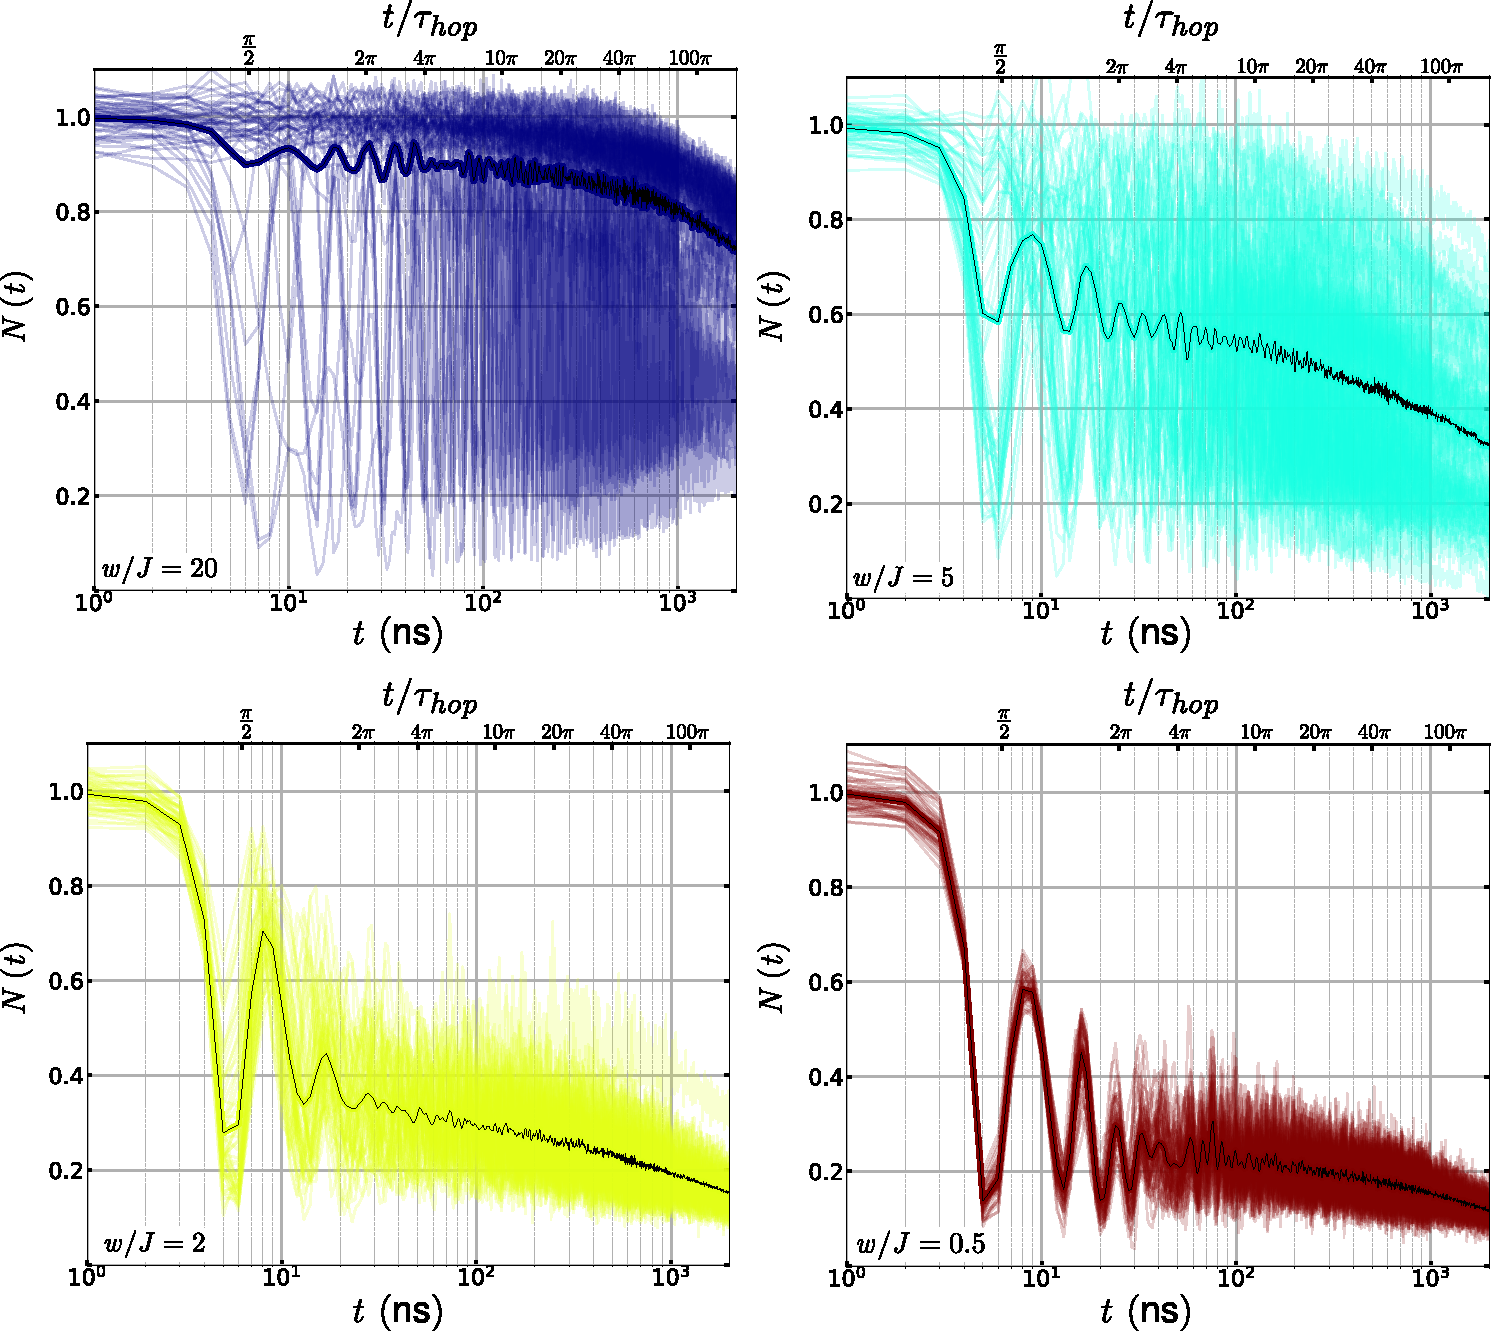
\includegraphics[width=0.8\textwidth, keepaspectratio]{./PDF/fs4_190625_150p.pdf}
        \caption{\textbf{Transport measurement instances.}
        Instances of $N \left( t \right)$ for the transport protocol prior to disorder averaging.
Data shown for $N_{ph}=2$ and selected values of disorder parameter $w$.
The disorder averaged data is contained in Fig. 2a, and the histograms in Fig. 2b are time slices of this data at $100 \, \text{ns}$.
The spread in values at short time is primarily due to readout error, as state preparation error is small.}
    \end{figure}

    \begin{figure}[tbh]
    \mutesubsection{Decoherence effects}
    \label{decoherence_effects}
    \centering
    \includegraphics[width=0.8\textwidth, keepaspectratio]{./PDF/fs5_190625_334p.pdf}%{./PDF/fig_sup_coherence_effects_190531_356p.pdf}
    \caption{\textbf{Transport Measurements:  Decoherence Effects.}
In the main text we report on short-time dynamics $t\lesssim 100 \, \text{ns}$, before our system is dominated by decoherence.
In reality, our $9$ qubit chain is an open system, subject to both relaxation and dephasing because of its coupling to the environment.
The characteristic relaxtion time $T_1$ is $\sim 10 \mu$s and the characteristic dephasing time is a few $\mu$s.
Here we provide additional data as an estimate of the importance of these open system effects.
In (a) we show the disorder averaged population vs time data for $N_{ph}=1$.
In (b) we show the population vs time data for $N_{ph}=1$ after correcting for relaxation (photon loss) using a simple single qubit $T_1$ model
$\overline{N^{corrected} \left( t \right)} = \overline{N \left( t \right)} / e^{\left( -t/10 \mu s \right) }$.
%
At high disorder, where the localization length is shorter than one lattice site,
single qubit $T_1$ (photon loss to the environment) is the dominant mechanism by which a photon leaves the observation site and this correction works well,
as indicated by the fact that the population has taken a stationary value.
%
At low disorder, in the diffusive regime, the excitations are able to distribute themselves evenly across the chain and we expect the $T_1$ correction to work well in this case as well.
Referring to Fig. 2c of the main text we see that at $100 \, \text{ns}$ in the diffusive regime at low disorder we measure the thermal expectation values.
This indicates clearly that relaxation effects are not significant in the first $100 \, \text{ns}$.
And that any apparent loss is due to transport within the $9$ qubit chain and not photon loss.
%
For intermediate disorders there appears to be additional photon loss, however this is actually dephasing assisted delocalization.\autocite{supplement,Znidaric2015, Levi2016, Fischer2016, Luschen2017, vanNieuwenburg2017}
When the LIOM extends over multiple lattice sites, dephasing between the sites breaks down the localized wave-packet by destroying the quantum interference pattern that causes the localization.
This breakdown of coherence between different parts of the wave packet enables transport of the excitation across the $9$ qubit chain.
Crucially, we note that neither $T_1$ relaxation nor dephasing between the lattice sites significantly influence the dynamics at higher disorders or short times.
This feature is captured in the main text fig. 5b where we note that $\overline{ \langle \sigma^{z} \rangle }$ is nearly constant between $10 \, \text{ns}$ and $100 \, \text{ns}$.
In (c) and (d) we show the raw and $T_1$ corrected data for $N_{ph}=2$.
}
    \end{figure}

    \begin{figure}[tbh]
        \mutesubsection{Two state occupation}
        \centering
        \includegraphics[width=0.8\textwidth, keepaspectratio]{./PDF/fs6_190625_312p.pdf}
        \caption{\textbf{Transport Measurements:  Two state occupation.}
        A critical feature of our system is that multiple excitations in the system may interact via the Hubbard interaction.
        The form of this interaction
        $H_{int} = \frac{U}{2}\sum\limits_{n=1}^{9} \,a^{\dagger}_{n}a_n(a^{\dagger}_{n}a_n-1)$
        indicates that it is only activated when there are multiple excitations on the same lattice site.
        Thus the interaction effects that we report in the main text require occupation of the higher levels of our Bose-Hubbard lattice.
        Here we report the $\ket{2}$ population vs time for a system initially in the state $\ket{\psi_0}=\ket{000000101}$ and observed on the right-most qubit.
        We find that the $\ket{2}$ state population is typically at the 2 \% level,
        achieves its maximum value early in the evolution, and does not progressively grow larger with time.
        }
    \end{figure}
\afterpage{\FloatBarrier}

%%%%%%%%%%%%%%%%  From Michael and Annabelle email 190508
\section{Interferometric protocols, Figs. S7-S9}
In order to gain some insights about the echo sequences, we first consider the case of very strong disorder, where the local integrals of motion (LIOMs) $\tau_i^z$ are close to the physical spins $S_i^z$ (represented by the two lowest energy levels of a qubit), and assume that we directly manipulate LIOMs. First, we will consider the spin echo sequence illustrated graphically in Fig. 7(a)~\cite{KnapPRL2014}.  Assuming we start from the vacuum state $\left|\psi_0\right> = \left| 0 \right>\otimes \ket{\{\tau_j\}} $, we initiate the dynamics by applying a $\pi/2$ pulse:
\begin{equation}
\ket{\psi} =\frac{1}{\sqrt{2}} (\ket{0} + i \ket{1}) \otimes \ket{\{\tau_j\}}
\end{equation}
When the system evolves for times $t/2$, the spin at site $i$ experiences an effective magnetic field, that depends on the states of the other LIOMs, see Eq. (2) in the main text,
\begin{equation}
\label{field}
\Delta_i = \tilde{h}_i  + \sum_j J_{ij} \tau_j^z + \sum_{j,k} J_{ijk}  \tau_j^z \tau_k^z + \ldots.
\end{equation}
\begin{figure}[b!]
\mutesubsection{Echo pulse sequences}
\centering
\includegraphics[width=.6\columnwidth]{./PDF/schem2}
\caption{\textbf{Interferometric Protocols:  Pulse sequences for spin and DEER echo.}}
\label{fig:4}
\end{figure}
The $\pi$ rotation halfway through the spin-echo sequence then inverts the effective magnetic field $\Delta_i \to -\Delta_i$ which is precisely canceled after another time evolution for $t/2$. At the end of the protocol we measure the purity, which is advantageous over measuring a single spin component, because it is less prone to running field gradients and external perturbations. For the spin-echo sequence on the LIOMs we find a perfect purity of one.
In a true measurement on our device the echo is performed on the physical spins, which possess a finite operator overlap with the LIOMs which is less than one. This leads to a spin echo signal that saturates to a finite value that decreases with decreasing disorder strength~\cite{KnapPRL2014}.

In the DEER echo sequence we similarly perform a spin echo measurement on site $i$ as before, However, half-way through the time evolution we modify a second part of the system, say site $j$ by applying a $\pi/2$ pulse, see
Fig. 7b. The effective magnetic field for the backward evolution $\tilde \Delta_i$, deviates from the field $\Delta_i$ of the forward evolution in all the terms containing $\tau_j^z$.
In summary, the state after the second time evolution is therefore
\begin{equation}
\ket{\psi_{D}(t)} = \frac{1}{2} \left[\ket{1}\otimes\ket{...0_j...} + e^{i (\Delta_i-\tilde{\Delta}_i) t - i\Delta_j t} \ket{1}\otimes \ket{...1_j...} - \ket{0}\otimes\ket{...0_j...}- e^{-i (\Delta_i-\tilde{\Delta}_i) t - i \Delta_j t} \ket{0}\otimes \ket{...1_j...}
\right]
\label{eq:deer_finaltime}
\end{equation}
and the measurement of the purity then yields
\begin{equation}
\tr \left(\rho^2\right) = \cos^2\left[\left(\Delta_i-\tilde{\Delta}_i\right) t\right].
\end{equation}
Due to the interaction between the $\tau$ bits at site i and j, the phases do not cancel anymore and the signal decays. The difference between spin and DEER echo is thus a pure interaction effect which would not appear in the noninteracting localized phase. The advantage of performing a differential measurement of the two echo protocols is that even in the presence of noise, deviations of the two echo signals, demonstrates a clear interaction effect and hence is able to unambiguously measure the interacting character of the LIOMs.
Because these interaction effects are due to the local occupation of higher orbitals we numerically estimate the population of multiply excited states $n_i^{max} = 1,2,3$ during the DEER echo protocol for a evolution time of $t = 63 \, \text{ns}$ in Fig.~\ref{figLocalOcc}.
In the experimental measurement of the purity, local occupations higher than two are not taken into account. This leads to a leakage of the measurement as characterized by the finite value of $\langle S^z_i\rangle$ in Fig. 4b of the main text. Moreover, we numerically estimate this effect by resolving the probabilities for maximum local occupations $n_i^{max} = 1,2,3$ during the DEER echo protocol for a evolution time of $t = 63 \, \text{ns}$ in Fig.~\ref{figLocalOcc}.
 From that it can be deduced that leakage effects are not severe, and in particular does not change the qualitative difference between the spin echo and DEER echo protocols.
%%%%%%%%%%%%%%%%%%%%%%%%%%%%%%%%%%%%%%%%%%%%%%%%%%%%%
\begin{figure}[h!]
\mutesubsection{Maximum local occupation}
\centering
\epsfig{file=./PDF/nimax_L9_N4_nmax3_J04_U16_mu4_tMax125_nReals50_nSReals1.pdf, width=0.49\textwidth}
\caption{\textbf{Interferometric Protocols:  Occupation of higher transmon levels during the DEER echo protocol.} Probability for maximum local occupations of $n_i^{max} = 1,2,3$ during the DEER echo protocol for $L=9$ sites, an evolution time of $T=63$ns, coupling $g=2\pi \cdot 40$MHz, disorder strength $w/g=10$ and interaction $U/g=4$.}
\label{figLocalOcc}
\end{figure}
%%%%%%%%%%%%%%%%%%%%%%%%%%%%%%%%%%%%%%%%%%%%%%%%%%%%%
%%%%%%%%%%%%%%%%  End From Michael and Annabelle email 190508


        %%%%%%%%%%%%%%%%%%%%%%%%
        %%%%%%%%%%%%%%%%%%%%%%%%  Discussion of Echo
        %%%%%%%%%%%%%%%%%%%%%%%%

        \begin{figure}
        \mutesubsection{Extended data}
        \centering
        \includegraphics[width=0.8\textwidth, keepaspectratio]{./PDF/fs9_190625_302p.pdf}%{./PDF/fig_sup_echo_extended_190612_355p.pdf}
        \caption{
        %Echo sequence to probe remote entanglement
        %Interferometric probe of entanglement.
        \textbf{Interferometric Protocols:  Extended Data.}
        \textbf{(a)} Spin and DEER echo pulse sequences.
        DEER echo differs from spin echo by the addition of a remote $\pi / 2$ pulse simultaineous with the spin echo $\pi$ pulse between the free precession intervals.
        \textbf{(b)} purity of the single qubit density matrix after the spin echo (dashed red lines) and DEER echo (solid lines) experiments.
        \textbf{(c)} $\left< \sigma^z \right>$ monitored over the echo experiments.
        %\textbf{(b)} and \textbf{(c)} are averaged over N instances of disorder.
        }
        \label{fig_3}
        \end{figure}
        \afterpage{\FloatBarrier}


\clearpage
\section{Logarithmic growth of entanglement in a small system (numerical analysis), Fig. S10}
In the main text we initialize the subsystem qubits into superposition in order to observe the development of entanglement.
Here we give numerical evidence to support that choice of initial state.
The growth of entanglement depends strongly on the choice of initial state.
Intuitively, since the system is localized and on-site population is constant,
we expect to observe the strongest entanglement growth by preparing the system into a phase sensitive initial state.

\begin{figure}[tbh]
\mutesubsection{numerical analysis}
\centering
\includegraphics[width=0.8\textwidth, keepaspectratio]{./PDF/log_growth_initial_state_numerics_mk_190612_458p.pdf}
\caption{
\textbf{Entanglement growth numerical study}
On a 6 site chain we perform numeric analysis to show the importance of initial state in the development of entanglement entropy.
In (a), we use an initial state that is analogous to the state chosen in the experimental work in the main text for figures 5b, 5c, and 6b.
In this case we observe entanglement growth consistent with the experimental observations.
There is a sharp increase in entanglement entropy during the first hopping interval,
followed by entanglement growth consistent with logarithmic time dependence before saturating at long times.
Panel (b) is initialized with excitations rather than superposition states and exhibits extremely weak entanglement growth after the first hopping interval.
This exemplifies the importance of the superposition state initialization in our detector region.
In (c) we initialize only the sites in the detection region into a superposition.
In this case there is no excitation on site 3 with which to interact and the entanglement growth and the entanglement growth is much weaker than in (a).
In (d) the first qubit is in a superposition state and there is one excitation outside the subsystem. Entanglement growth is reduced compared to (a) because interactions kick in only at exponentially later times giving rise to an intermediate plateau.
In (e) all qubits are initialized into superposition states and the system becomes rapidly entangled.
In (f) every other qubit is in a superposition state and the system accumulates entanglement continuously, although not as rapidly as in (e) (please note the different y-axis scales).
In (g) with every other qubit initialized into an excitation state there is only extremely weak growth of entanglement after the first hopping time scale.
}
\label{log_growth_initial_state_numerics}
\end{figure}
\afterpage{\FloatBarrier}


%%%%%%%%%%%%%%%%  From Michael and Annabelle email 190508
\section{Entanglement Measures}
The distillable entanglement of the two qubit density matrix $E_D(\rho_{2q})$ is lower bounded by the coherent information entropy
\begin{equation}
E_D(\rho_{2q}) \geq S(\rho_{1q}) - S(\rho_{2q}),
\end{equation}
where $\rho_{1q,2q}$ are the reduced density matrices of one of the two qubits and the two qubit subsystem, respectively, and $S(\rho)$ is the von Neumann entanglement entropy.
An upper bound to the distillable entanglement is provided by the logarithmic negativity\autocite{Vidal2002} which is defined as
\begin{equation}
E_N(\rho_2) = \log_2 || \rho_2^{T_A} ||_1.
\end{equation}
Here, $\rho_2^{T_A}$ is the partial transpose of the reduced density matrix with respect to one of the qubits and $|| \cdot ||_1$ denotes the trace norm.

A second operational entanglement measure is the entanglement of formation, which is a measure for the entanglement needed to create a given entangled state\autocite{Wootters1998}.
It is defined as
\begin{equation}
E_F(\rho) = \epsilon(\mathcal{C}(\rho))
\end{equation}
with
\begin{equation}
\epsilon(x) = -h_+(x) \log_2 h_+(x) - h_-(x)\log_2 h_-(x)
\end{equation}
where
\begin{equation}
h_{\pm}(x) = -\frac{1}{2} \left(1\pm \sqrt{1-x^2} \right).
\end{equation}
The concurrence $\mathcal{C}(\rho)$ of a mixed state of two qubits is defined as
\begin{equation}
\mathcal{C}(\rho) = \max \left(0,\lambda_1-\lambda_2-\lambda_3-\lambda_4\right),
\end{equation}
where $\lambda_i$ are the eigenvalues of
\begin{equation}
R = \sqrt{\sqrt{\rho}\tilde{\rho}\sqrt{\rho}}
\end{equation}
and
\begin{equation}
\tilde{\rho} = (\sigma_{y}\otimes\sigma_{y})\rho^{*}(\sigma_{y}\otimes\sigma_{y}).
\end{equation}
%%%%%%%%%%%%%%%%  From Michael and Annabelle email 190508
\renewcommand*{\bibfont}{\scriptsize}
\printbibliography

\clearpage
%\input{./currently_excluded.tex}
\clearpage
%\input{./supplement_todo_list.tex}
\end{document}
